\documentclass[thesis.tex]{subfiles}
\begin{document}
\chapter{Towards AppPAL Applications and Extensions}
\label{chap:extensions}

So far we have described the policies of the mobile
ecosystem and how AppPAL can be used to describe them.  We have argued
that AppPAL is a good language for describing these policies, however
there are also areas where AppPAL could be improved to further to
describe more kinds of policies and to aid policy authors.  This
chapter looks at two such areas and describes our
explorations.  We describe how AppPAL policies can
be analyzed automatically and describe an early prototype to check
policies for common problems.  We also describe
how plausibility, quantified doubt, could be used to express
confidence in a statement in an AppPAL policy.


\section{Plausible AppPAL}

\newcommand{\secpalmath}[1]{\ensuremath\texttt{#1}}
\newcommand{\AC}[0]{\ensuremath\text{AC}}
\newcommand{\says}[1]{\ensuremath~\secpalmath{says}^{\new{#1}}~}
\newcommand{\canSay}[1]{\secpalmath{can-say}_{#1}}
\newcommand{\canActAs}[0]{\secpalmath{can-act-as}}
\newcommand{\spif}[0]{\secpalmath{if}}
\newcommand{\where}[0]{\secpalmath{where}}

The SecPAL authorization language, and the AppPAL instantiation, allow
policy authors to make use of static analysis tools to make decisions,
and allow principals to make statements about apps through delegation.
When these decisions are made they are made with certainty.  If a
principal says an app is safe to access the network then we believe
that that principal definitely believes the app is safe on a network.
When a static analysis tool finds that an app isn't malware then we
believe that app to not be malware.  This isn't realistic.  Static
analysis tools can produce false results.  A principal might be merely
fairly confident that an app can access the network safely but not absolutely
certain.

With current authorization languages you cannot quantify the belief a principal
has in any statement. A principal cannot say how \emph{plausible} they think any
statement is.

\subsection{Examples of Plausibility}

SecPAL was designed to make access control decisions. The decision whether to
install allow a user access to a file or not is a binary one: either they can
access it or they cannot. Similarly the decision process for these decisions is
also binary: a user is either logged in or not, a network address is either in
the network or outside it, someone can act as someone else's manager or they can
not. Not all decisions are binary however.

\begin{figure}
  \centering
  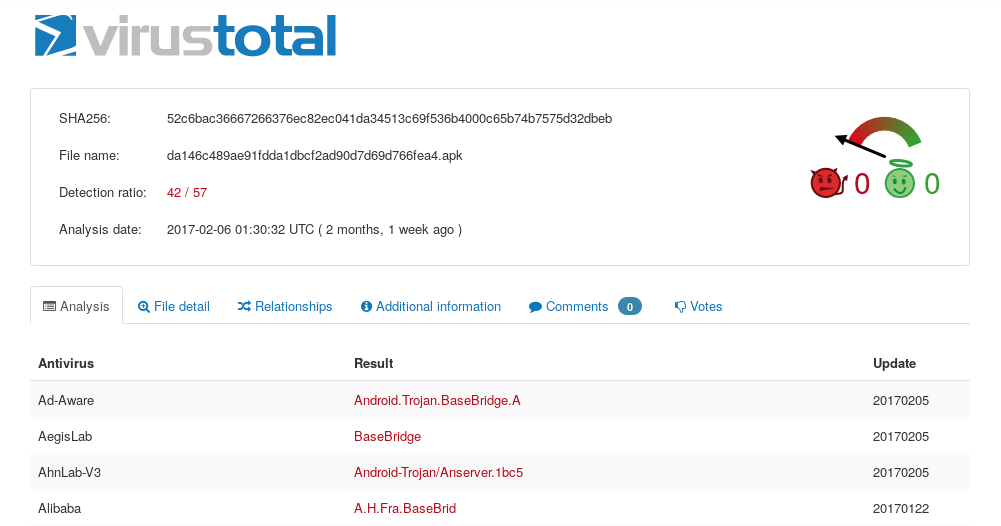
\includegraphics[width=0.49\linewidth]{figures/android-malware.png}
  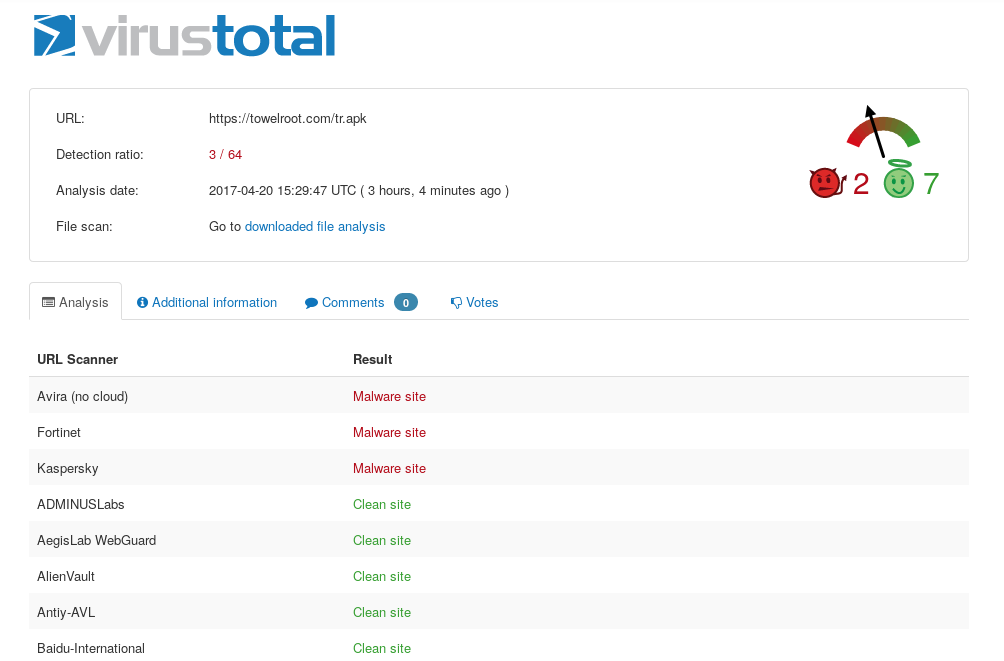
\includegraphics[width=0.49\linewidth]{figures/towelroot.png}
  \caption[VirusTotal results for two Android apps.]{VirusTotal results for 57
    antivirus packages scanning a sample of the BaseBridge Android malware, and 64
    antivirus packages analyzing a download of the (relatively safe) Towelroot
    rooting app.}
  \label{fig:android-malware}
\end{figure}

A user, Alice, may have a policy. That will only install safe apps, ones they
know are not malware. She could use an \ac{AV} program, but these tools are not
infallible. Some change their mind about apps over time. Others are heuristic
based and may only be capable of judging an app based on sufficiently many
malware indicators being present. Instead of using one \ac{AV} program, Alice
opts to use \emph{VirusTotal}; a webservice for running files through multiple
\ac{AV} programs. Even for known malware samples VirusTotal rarely gives
absolute answers instead giving the number of \ac{AV} programs that flagged
it~(\autoref{fig:android-malware}). Alice acknowledges this and writes her
policy accordingly:

\begin{lstlisting}
'alice' says App:A isInstallable
  if A isSafe
  with plausibility at least 0.75.

'alice' says 'virustotal' can-say
  App:A isSafe

'virustotal' says 'com.good.app' isSafe
  with plausibility 0.95.

'virustotal' says 'com.malicious.app' isSafe
  with plausibility 0.26.
\end{lstlisting}

She can install the \texttt{com.good.app}, since the plausibility it is good is
greater than her threshold but the \texttt{com.malicious.app} fails her test and
is uninstallable. 

In the first example VirusTotal gave Alice a value for how plausible it was the
app was safe: but what if Alice has to decide this value herself? An example of
this is app recommendations. Alice only wants to install apps that are really
good. She has two friends, Bob and Charlie, who offer her reviews of a game. To
complicate matters further, whilst she trusts Bob utterly, she is a little less
trusting of Charlie.

\begin{lstlisting}
'alice' says App:A isInstallable
  if A isGood
  with plausibility

'bob' says 'com.rovio.angrybirds' isGood
  with plausibility 0.8.

'charlie' says 'com.rovio.angrybirds' isGood
  with plausibility 0.9.

'alice' says 'bob' can-say App:A isGood.

'alice' says 'charlie' can-say App:A isGood
  with plausibility 0.9.
\end{lstlisting}

How should she combine the information to get an overall rating of the game? If
Alice wants to only install an apps that are both good and safe how should she
trade off the plausibility against each other? Is she willing to install a more
dangerous app if it is highly reviewed?



Probabilistic versions of Datalog are not a new idea.  Various papers proposed
probabilistic variants of Datalog~\cite{fuhr_probabilistic_1995} or explored the
semantics of probabilistic logics~\cite{halpern_analysis_1990}.  Role-based
access control languages have incorporated ideas about risk into their
schemes~\cite{josang_analysing_2004,dimmock_using_2004,salim_approach_2011},
which is a similar notion to plausibility and trust.  These schemes do not seem
to deal with delegation in the same manner as SecPAL however so incorporating
similar ideas here may be interesting and allow SecPAL and AppPAL greater
expressiveness.  Part of the work toward this this year has included modifying Becker's
evaluation and translation-to-Datalog algorithms~\cite{becker_secpal:_2010} to
include a plausibility value, and for giving rules to query on the basis of
them, using Datalog$^C$~\cite{li_datalog_2003}.

\subsection{Modifying AppPAL for Plausibility}

AppPAL has three rules for evaluation: \emph{cond}, \emph{can-say},
and \emph{can-act-as}.  We modify the language so that the \emph{says}
keyword has an an annotation $0 \geq p \geq 1$ denoting a statements
\emph{plausibility}.  If the annotation is missing then it is assumed
to be $1$ We also assume a plausibility combining function $\oplus$
which combines plausibility.  The AppPAL inference rules then become
as follows, with additions highlighted in \new{red}.

{\footnotesize\centering
\begin{equation*}
  \infer[\text{cond\new{$\leq$}}]{
    \AC{}, D \models A~\says{\bigoplus_{i=1}^n p_i}~f\theta
  }{
    \begin{matrix}{
      \left(A~\says{}~f~if~f_1\cdots f_n~\where~c~\new{\text{with plausibility at least}~p_{lim}}\right) \in \AC{}
    }\\{
      \forall i \in [1\cdots n]. \AC{}, D \models A~\says{p_i}~f_i\theta
    }\\\new{
      0 < p_{lim} \leq \bigoplus_{i=1}^n p_i
    }
    \end{matrix}&
    \vdash c\theta &
    vars\left(f\theta\right) = \emptyset
  }
\end{equation*}
\begin{equation*}
  \infer[\text{cond\new{=}}]{
    \AC{}, D \models A~\says{p_{lim}}~f\theta
  }{
    \begin{matrix}{
      \left(A~\says{}~f~if~f_1\cdots f_n~\where~c~\new{\text{with plausibility is}~p_{lim}}\right) \in \AC{}
    }\\{
      \forall i \in [1\cdots n]. \AC{}, D \models A~\says{p_i}~f_i\theta
    }\\\new{
      0 < p_{lim} \leq \bigoplus_{i=1}^n p_i
    }
    \end{matrix}&
    \vdash c\theta &
    vars\left(f\theta\right) = \emptyset
  }
\end{equation*}
\begin{equation*}
  \infer[\text{can-say}]{
    \AC{}, \infty \models A~\says{p_1 \oplus p_2}~f
  }{
    \AC{}, \infty \models A~\says{p_1}~B~\canSay{D}~f &
    \AC{}, D \models B~\says{p_2}~f
  }
\end{equation*}
\begin{equation*}
  \infer[\text{can-act-as}]{
    \AC{}, D \models A~\says{p_1 \oplus p_2}~x~vp
  }{
    \AC{}, D \models A~\says{p_1}~x~\canActAs~y &
    \AC{}, D \models B~\says{p_2}~y~vp
  }
\end{equation*}
\begin{equation*}
  \new{
    \infer[\text{reduce}]{
        \AC{}, D \models A~\says{p}~f
    }{
        \AC{}, D \models A~\says{p^\prime}~f & p \leq p^\prime
    }
  }
\end{equation*}
}

In general any derived statement is at most as plausible as the
combination of the statements that went into deriving it.  We split
the \emph{cond} rule into two variants.  The \emph{cond$\leq$} rule
allows us to specify a minimum plausibility required by combining all
the conditional statements and if that limit is exceeded we take the
combined probability in the plausibility of the outcome.  The
\emph{cond=} rule allows us again to set a minimum plausibility but
this time we take the stated plausibility if the rule is satisfied.
These two \emph{cond} rules serve different purposes.  The
\emph{cond=} variant is useful when we want to set a limit on the
plausibility: for instance when we have a tool with a known confidence
rate we want to run, or a fact which we know how plausible it is.  The
\emph{cond=} rule is useful for when you want to ensure that a
decision is made with a certain least-confidence, for instance if you
want to be at least 80\% sure that an app is safe to use before doing
anything with it.  In this case we would want the combined
plausibility to trickle through the proof not the lower limit.

We also add a plausibility reduction rule that allows us to reduce the
plausibility of an assertion, this allows us to phrase a policy query
as \emph{``is it at least 50\% plausible that...''} rather than having
to discover the plausibilities precisely.

\subsubsection{Plausibility Combination}

How should the plausibility combination operator be defined?  One
simplistic approach might be to take the least plauable assertion as
the final value.  This however is too simple. Consider the case where
an app needs to be safe and from a reputable developer.  Say we're
50\% sure the app is safe but we are unsure of the developer. We are
90\% sure Google is reputable and only 60\% sure Rovio is.  No matter
who the developer is the combined probability is the same (50\%) so
the distinction is lost.

\begin{equation*}
  p_a~\oplus_{\text{min}}~p_b~\gets~\text{min}~p_a~p_b
\end{equation*}

If we are sure the plausibilities are independent we could multiply
them together to get the final plausibility. This is appealing in that
if we take the example above if Google is the developer we're 45\%
sure the app is usable, but only 30\% if Rovio is.  If however there
are a lot of combinations to be made the probabilities may get very
small and be difficult to distinguish.

\begin{equation*}
  p_a~\oplus_{\text{ind}}~p_b~\gets~p_a\times p_b
\end{equation*}

Both the two previous suggestions are na\"ive in their approach.  The
first is unnecessarily conservative, the second assumes independence.
A better scheme may be to incorporate a more sophisticated reasoning
system.  One system might be Dempster-Schafer
theory~\cite{dempster_upper_1967,glenn_shafer_mathematical_1976} which
is designed to reason about the probability of provability of any
statement. It can also be used to give a value to how close evidence
comes to rendering a proposition
provable~\cite{pearl_probabilistic_2014}. Other schemes, and working
out how to implement and integrate this into AppPAL is left to future work.

\subsection{Guarantees for Plausible AppPAL} 

However plausibility combination is implemented some thought should be
given to what properties and guarantees AppPAL ought to offer.  One
guarantee might be that if all statements are perfectly plausible then
this ought to be equivalent to standard AppPAL.  Another might be that
if a statement is perfectly implausible then it ought to be equivalent
to the statement not existing at all. A third rule should be that we
can't make a statement more plausible by combining less plausible
statements.  To summarize:

\begin{itemize}
\item If all statements have a plausibility of $1$, then this is
  equivalent to standard AppPAL.
\item If a statement has a plausibility of $0$, then it is equivalent
  to the statement not existing in the assertion context.
\item No statement should be more certain than the conditionals used
  to derive it.
\end{itemize}

Point 1 is true since if $p_{\text{lim}} = 1$ then no statement will
be accepted unless its plausibility is also 1.  If we combine the
plausibility of two events this will also be 1 (using either method
described so far): hence the restriction on the plausibility in the
cond rule is always true since all statements have a plausibility of
one.  Rewriting the rules with this in mind we get the original AppPAL
inference rules, so if all statements have a plausibility of 1, then
this must be equivalent to standard AppPAL.

Point 2 is also true by the restriction on probabilities in the cond
rule.  Since $p_{\text{lim}}$ must be greater than 0, if a statement
has a plausibility of 0 then it will not be accepted.  Similarly when
combining plausibilities if a statement is completely inplausible then
the plausibility of it happening with another event must also be
implausible.  Hence the combination should always be 0, and no
statement combined with an implausible statement will be derivable.

Point 3 is important as we don't want a means to make a statement more
certain by repeatedly applying a rule.  For example imagine we had a
combination operator that took the sum (or 1 if the combination was
greater than 1), and a rule such as:

\begin{lstlisting} 
'x' says 'y' p if 'y' p, 'y' p.
\end{lstlisting}

If we also have statement that $x \says{0.2} y p$,
then we could apply this rule to get $x \says{0.4} y p$, and so on
until we're certain.

Similarly if we had statements  such as:
\begin{lstlisting} 
'x' says 'y' p 
  if 'y' p,
     'z' p.
\end{lstlisting}

If we knew, with certainty, that \lstinline!'x' says 'z' p!, then if
we used a plausibility combination function that averaged the
plausibilities we would increase the overall plausibility that
\lstinline!'x' says 'y' p.!

The multiplication and minimum plausibility rules won't allow you to
increase plausibility like this (minimum is trivial: if it is always
the plausibility of the least plausible statement then plausibilities
will never increase; multiplication works because if all
plausibilities are between 1 and 0, then the product will also never
increase).

\end{document}

%%% Local Variables:
%%% mode: latex
%%% TeX-master: "../ch6.tex"
%%% End:
